Neste capítulo é mostrada uma proposta de abordagem a este problema através de uma aplicação a qual tem se como objetivo facilitar o acesso a dados públicos de forma facilitada através de linguagem natural.

\section{\uppercase{Estudo a respeito do Elasticsearch}}
Para busca e persistência dos dados será utilizada a tecnologia \textit{Elasticsearch}, que se caracteriza por ser um conjunto de mecanismo de busca \textit{open-source} que realiza buscas e analisa dados em tempo real \cite{Gil:2010}. Através disso, são criada soluções próprias que utilizam as  facilidades trazidas pelo conjunto para atingir seus objetivos.

Tendo como principal objetivo facilitar a busca por texto e a rapidez no acesso aos dados e gravação, o \textit{Elasticsearch} possui a capacidade de funcionamento escalável, sendo possível a utilização em apenas um servidor (\textit{standalone}) ou de forma distribuída em centenas de servidores \cite{Gormley:2015}, agilizando assim a entrega ao usuário ou aplicação que solicitar os dados persistidos.

Para solicitar os dados persistidos é disponibilizada uma interface RESTful API que possibilita a obtenção e visualização dos dados por aplicações \textit{web client} \cite{Gormley:2015}. Esta funcionalidade disponibiliza a comunicação entre o \textit{Elasticsearch} e outras aplicações independentemente de como foram feitas ou da linguagem utilizada na construção das aplicações \textit{web clients}. Gera-se assim, independência e maior usabilidade.

Possuindo como base o \textit{Apach Lucene}, o qual se qualifica por ser atualmente a livraria de motor de busca mais avançada, performática e completa  existente, o Elasticsearch é construído na linguagem Java para poder integrar e usufruir dessa livraria. Ao contrário, é necessário um grande volume de conhecimento para compreender como são realizada as facilidades trazidas pelo \textit{Lucene} devido a sua complexidade \cite{Gormley:2015}.

Um dos maiores benefícios trazidos pela da utilização do \textit{Apach Lucene} é a ação de indexação. Utilizando isso, o \textit{Elasticsearch} realiza busca, ordena, filtra e persiste dados fornecidos como objetos e documentos realizando a indexação em todas as suas ações. Consequentemente, esta tecnologia também é caracterizada como orientada a documento \cite{Gormley:2015}.

Um documento é um dado constituído por campos os quais pode se repetir várias vezes. Todos os campos possuem um tipo como texto, numérico, data etc., ou tipos mais complexos como subdocumentos ou \textit{arrays}. Para cada documento persistido é salvo um pequeno título, data de publicação e um \textit{link} de acesso ao conteúdo. O ato de se persistir um documento é chamado de indexação e o nome do dado persistido é chamado de índice \cite{Kuc:2013}.

Após a criação desta estrutura, é possível realizar pesquisas através de temas. Agilizando assim, a obtenção dos dados desejados. A disponibilização dos dados solicitados ocorre através de uma simples API RESTful mediante a transformação e transporte dos dados no formato \textit{JavaScript Object Notation}(JSON) como exemplificado na \autoref{pretty}.


\begin{figure}[!htb]
	\caption{\label{pretty}JSON - Resposta da chamada a API. Comando: curl http://localhost:9200/?pretty}
	\begin{center}
		%\includegraphics[width=\textwidth, height=\textheight]{imagens/pretty.eps}
		\includegraphics[width=0.5\textwidth, height=0.35\textheight]{imagens/pretty.eps}
		%\includegraphics[width=0.7\textwidth]{imagens/pretty.eps}
	\end{center}
	\legend{Fonte: Autor}
\end{figure}
%\clearpage

\section{\uppercase{Inteligência Artificial}}
Inteligência Artificial é uma das ramificações da ciências computacionais que se dedica ao estudo de tentar simular a inteligência humana em maquinas, desenvolver a inteligência artificial de máquinas e softwares que podem raciocinar, aprender, reunir conhecimento, comunicar, manipular e perceber objetos. Inteligência é comumente considerado como a capacidade de resolver problemas complexos realizando previamente coleta de informações e conhecimentos \cite{Pannu:2015}.

\noindent \marcador{Em um futuro próximo, máquinas inteligentes substituirão humanos com as mais diversas capacidades em várias áreas, com isso a inteligência artificial pode ser resumida em estudo e desenvolvimento de máquinas inteligentes e software que pode raciocinar aprender, reunir conhecimento, comunicar, manipular e perceber objetos.}

\subsection{Processamento de Linguagem Natural (PLN)} Processamento de Linguagem Natural (PLN) é uma subárea da Inteligência Artificial (IA) que estuda as limitações, problemas e compreensão da linguagem humana para resoluções de problemas solúveis através de uma inteligência artificial.  Seu objetivo principal é possibilitar maquinas entenderem e interpretarem a linguagem humana. Tal processo converte dados em texto em formatos que máquinas entendam como o numérico e binário \cite{Kulkarni:2019}.

Este processo é baseado em quatro etapas para extrair informações pertinentes do texto alvo. Primeiro o texto é realizado um processo que criação de \textit{tokens} das palavras do texto. Nesta etapa o texto é quebrado em unidades, sem se preocupar no significado ou classificação gramatical das palavras. Formando assim uma lista de \textit{tokens} que será usada em todos os outros processo com seus diferentes objetivos \cite{Reese:2015}.

A segunda etapa é dedicada a detecção de sentenças utilizando unidades criados na primeira etapa. A combinação de palavras em uma frase ou uma sentença pode ter diferentes significados mudando o relacionamento entre outras palavra ou outras sentenças. Pode ser dado como exemplo que, frequente é distinguido a função gramatical entre as palavras como substantivo e verbos \cite{Reese:2015}.

A terceira é o processo de classificada cada palavra e documentos que consiste na rotulação destas informações encontradas no texto. No processo de rotulação, o rótulo pode ou não existir antes desta etapa. Caso exista, esta etapa é chamada de classificação. Antagônico, é chamado de agrupamento \cite{Reese:2015}.

A quarta etapa é o processo de extração de relacionamentos identificado no texto.
Relationship extraction
relationships exist in text
humans can determining how things are related to each other


\section{\uppercase{Estudo a respeito da Language Understanding Intelligent Service}}
Language Understanding Intelligent Service (LUIS) é uma suite de \textit{software} pertencente a um dos Serviços Cognitivos da Microsoft que utiliza um ramo da Inteligência Artificial (IA) chamado Processamento de Linguagem Natural (PLN).

O objetivo de utilização desta ferramenta é possibilitar a tradução de linguagem natural em texto plano para que programas de computadores possam entender e interagir utilizando tais dados. Para isso, a API extrai de uma sentença dada as intenções e entidades retornando objetos no formato JavaScript Object Notation (JSON) \cite{Mayo:2017}.

É necessário, anteriormente, a criação de modelos de linguagens os quais possibilitam o reconhecimento de intenções e entidades em uma entrada do usuário. Seja esta entrada uma frase ou um texto em linguagem natural.

